\documentclass[a4paper]{article}
\usepackage{amsmath,amssymb,enumerate, graphicx,amsfonts, makeidx, hyperref}
\renewcommand{\labelitemi}{\tiny$\blacksquare$}

\usepackage{listings}
\lstset{language=C}
\begin{document}
\begin{center}
{\bf{\huge CS 241 }}\\
{\bf{\huge a.k.a. System Programming}}\\
\vspace{ 5 cm }
{\bf{\large Spring 2012, University of Illinos}}\\
{\bf{\large as taught by Brigthen Godfrey}}\\
\vspace{ 1 cm }                         
{\large notes by Michele R. Esposito}\\
\vspace{ 5cm }
Please, let report any error or type-o at \underline{\href{mailto:micheleresposito@gmail.com}{ micheleresposito@gmail.com }}

\end{center}

\newpage
\tableofcontents
\newpage
\begin{center}
{\bf{\huge Study Guide Midterm }}\\
CS 241 \\
Spring 2012 \\
Created by Michele Esposito\\
\end{center}

% =========================================================
\section{C Programming} % (fold)
\label{sec:C Programming}
\subsection{What is POSIX} % (fold)
\label{sub:What is POSIX}
POSIX is the UNIX Interface Standard. It is a family of standards specified by the IEEE for maintaining compability between
OSs. POSIX defines the application programming interface (API) along with command lines shells and utility interfaces, for software
compatible with variants of UNIX and other operating systems. It includes:
\begin{itemize}
  \item Process: creation and control
  \item Signals
  \item Floating point exceptions
  \item Segmentations
  \item C Library
  \item Timers
  \item Priority scheduling
  \item Shared Memory
  \item Semaphores
  \item Thread creation, control and cleanup
  \item Thread scheduling
  \item and much more $\dots$.
\end{itemize}
% subsection What is POSIX (end)
\subsection{Explain the difference between a library function and a system call} % (fold)
\label{sub:Explain the ≠ between a library functino and a system call}
{\bf System Calls}
A syscall is a request to the OS to perform some activity. They are expensive, as the system needs to perform the following operations:
\begin{itemize}
  \item The hardware save its state
  \item The OS code takes control of the CPU, privileges are updated
  \item The OS examines the call parameters
  \item The OS performs the requested function
  \item The OS saves its state (and call results)
  \item The OS returns control of the CPU to the caller
\end{itemize}
A call to a library function can be anything like $printf$, that does not necessarily require a syscall. This is just like a
normal C function, only comes from an external library.
% subsection Explain the ≠ between a library functino and a system call (end)
\subsection{Give an example of a POSIX system call used in CS241 lectures or reading.} % (fold)
\label{sub:Give an example of a POSIX system call used in CS241 lectures or reading.}
fprintf, fclosef, pthread-create. There are a loot!
% subsection Give an example of a POSIX system call used in CS241 lectures or reading. (end)
\subsection{What is the * operator? What does it do? What is the $\&$ operator? What does it do?} % (fold)
\label{sub:subsection name}
The * operator is the dereference operator. When you use it, it looks up the memory inside the address of your variable. \\
The $\&$ is the address operator. When you use it tell you the address of your variable.
% subsection subsection name (end)
\subsection{How do you define a function pointer?} % (fold)
\label{sub:How do you define a function pointer?}
A function pointer is a pointer which points to the address of a function. 
% subsection How do you define a function pointer? (end)
\subsection{What is the difference between a global and a static variable?} % (fold)
\label{sub:What is the difference between a global and a static variable}
Static variables are local in scope, but their life is for the entire program. Globals instead have global scope. 
% subsection What is the difference between a global and a static variable (end)
% section C Programming (end)
% =========================================================
\section{Memory} % (fold)
\label{sec:Memory}
\subsection{Key concepts} % (fold)
\label{sub:Key concepts}
\begin{itemize}
  \item {\bf Virtual memory}
    \begin{itemize}
      \item Memory addresses used by an application
      \item Unrelated to physical address
      \item May not even be stored in physical memory
    \end{itemize}
  \item {\bf Physical memory}
    \begin{itemize}
      \item The RAM in my computer
    \end{itemize}
  \item {\bf Memory Management Unit (MMU)}
    \begin{itemize}
      \item Hardware which translates virtual to physical addresses every time any program accesses any memory
    \end{itemize}
  \item {\bf Page}
    \begin{itemize}
      \item Unit in which OS allocates memory to applications
      \item MMU also works in units of page
    \end{itemize}
  \item {\bf Page table}
    \begin{itemize}
      \item DS used by MMU to remember virtual-to-physical mapping
      \item One per process
      \item Created by OS, stored in memory (at least top level)
    \end{itemize}
  \item {\bf Translation Lookaside Buffer (TLB) }
    \begin{itemize}
      \item Cache of virtual-to-physical mappings
      \item Faster than extra memory references needed to look up in page table
      \item Must be flushed when switching between apps
    \end{itemize}
  \item {\bf Multilevel page table }
    \begin{itemize}
      \item Top level page table points to other page tables rather than individual pages
    \end{itemize}
  \item {\bf Segmentation fault }
    \begin{itemize}
      \item Program accesses memory outside the segment that it is allowed to access
        \begin{itemize}
          \item defer. NULL pointer
          \item write past end of heap $\dots$
        \end{itemize}
    \end{itemize}
  \item {\bf Page faults}
    \begin{itemize}
      \item Happen when the VP is not currently mapped to a valid physical page
      \item Seg fault is one kind of page fault
    \end{itemize}
\end{itemize}
% subsection Key concepts (end)
\subsection{What is the difference between physical and virtual memory?} % (fold)
\label{sub:What is the difference between physical and virtual memory?}
Physical memory is the actual memory on the machine, which is made of the HD, RAM and caches. Virtual memory instead
is an illusion created so that the program can think it has an infinite amount of resources to draw from. it just adds a very important level of abstraction about dealing with memory.
% subsection What is the difference between physical and virtual memory? (end)

\subsection{What are the different mem allocation algorithms, and what are the advantages to each?} % (fold)
\label{sub:What are the ≠ mem allocation algorithms, and what are the advantages to each?}
\begin{itemize}
  \item {\bf Implicit Free List}
    \begin{itemize}
      \item Idea: Each block contains a header w some extra information
      \item Allocated bit indicates free or not.
      \item Size field indicates entire size of block ( w header)
      \item No explicit structure tracking location of free/allocated blocks
      \item $O(n)$ worst case to allocate a free block.
      \item $O(n)$ to coalesce.
      \item \underline{Summary}
        \begin{itemize}
          \item {\bf Implementation}: very simple.
          \item {\bf Allocate:} linear-time worst case.
          \item {\bf Free:} Linear-time worst case even with coalescing.
          \item {\bf Memory usage}: depends on placement policy.
        \end{itemize}
    \end{itemize}

  \item {\bf Explicit Free Lists}
    \begin{itemize}
      \item Use doubly liked listed, with boundary tags for coalescing, to keep track of free blocks.
      \item Efficiency depends on insertion policy.
    \end{itemize}
  \item {\bf Buddy Allocators}
    \begin{itemize}
      \item Special case of segregated fits
      \item Divide into lists of powers of two.
      \item \underline{Advantages}: minimizes external fragmentation
      \item \underline{Disadvantages}: internal fragmentation when not $2^{n}$ sized request.
    \end{itemize}
\end{itemize}
% subsection What are the ≠ mem allocation algorithms, and what are the advantages to each? (end)
\subsection{How are VA transelated to physical addresses in multi-level page table?} % (fold)
\label{sub:How are VA transelated to physical addresses in multi-level page table?}
Starting from the VA, we have the following steps:
\begin{enumerate}
  \item The CPU sends the VA to the MMU
  \item The MMU decomposes the address, and sends the VPN to the TLB.
  \item If TLB hit, then PA is send to the memory, data is returned
  \item If TLB miss, then:
    \begin{enumerate}
      \item MMU looks up index in primary PT, to get secondary page table
      \item MMU tries to access secondary PT.
      \item MMU looks up index in secondary PT to get physical frame $\#$.
    \end{enumerate}
\end{enumerate}
% subsection How are VA transelated to physical addresses in multi-level page table? (end)
\subsection{How does page size and the number of levels of page tables affect the number of entries in a page table?} % (fold)
\label{sub:How does page size and the number of leverls of page tables affect the number of entries in a page table?}
The more levels you have, the more number of entries you are allowed, as you have another level of indirection, which allows
you to have more and more page. However, too many levels are a problem. The page size does not really effect.
% subsection How does page size and the number of levels of page tables affect the number of entries in a page table? (end)
\subsection{What is the difference between internal and external fragmentation?} % (fold)
\label{sub:What is the ≠ btw internal and external fragmentation?}
\begin{itemize}
  \item External fragmentation
    \begin{itemize}
      \item Unused chunks of memory between allocated chunks
      \item Can't use for large contiguous allocations
    \end{itemize}
  \item Internal fragmentation
    \begin{itemize}
      \item Unused memory within allocated regions
      \item Because we have allocated more than the requested
    \end{itemize}
\end{itemize}
% subsection What is the ≠ btw internal and external fragmentation? (end)
\subsection{What is the ≠ btw MMU and TLB?} % (fold)
\label{sub:What is the ≠ btw MMU and TLB?}
The MMU is a hardware unit that transelates the $VA \rightarrow PA$. However, this process is expensive, and it takes a long time to complete.
A TLB, transelation lookaside buffer, is a cache for the MMU. Like that, the MMU will only need to compute the address once, and then it will be saved in the system.
% subsection What is the ≠ btw MMU and TLB? (end)
\subsection{What are different page replacement policies and teh advantages of each?} % (fold)
\label{sub:What are different page replacement policies and teh advantages of each?}
The goal of the page replacement algorithm is to evict the best page possible, which are those that will never be used
again in the system. \\ 
{\bf Algorithms} 
\begin{itemize}
  \item {\bf OPT a.k.a. MIN}
    \begin{itemize}
      \item Evict page that won't be used for the longest time in the future.
      \item This requires to see the future, thus it cannot be implemented.
      \item It is only a benchmark.
    \end{itemize}
  \item {\bf Random:} Throw out a random page. Not the best scheme $\dots$
  \item {\bf FIFO:} Throw out pages in the order that they were allocated.
    \begin{itemize}
      \item Maintain a list of allocated pages.   
      \item When the length of hte list grows, pop first page off list and allocate it.
      \item \underline{Advantages:} Maybe the page allocated very long ago isn't used anymore.
      \item \underline{Disadvantages:}
        \begin{itemize}
          \item Doesn't consider locality.
          \item Suffers Belady's anomaly: Performance of a n app might get worste as the size of physical memory increases!
        \end{itemize}
    \end{itemize}
  \item {\bf Least Recently used (LRU)}
    \begin{itemize}
      \item Evict the page that was used the longest time ago.
        \begin{itemize}
          \item Keep track of when pages are referenced to make a better decision
          \item Use past behaviour to predict future behavior
        \end{itemize}
      \item Implementation
        \begin{itemize}
          \item Every time a page is accessed, record a timestamps of the access time
          \item When choosing a page to evict, scan over all pages and throw out page with oldest timestamps
        \end{itemize}
      \item \underline{Issues:}
        \begin{itemize}
          \item Not Optimal
          \item Requires lot of space for time stamp.
        \end{itemize}
      \item \underline{Approx. LRU}
      \begin{itemize}
        \item Use a counter to keep track of the LRU.
      \end{itemize}
    \end{itemize}
\end{itemize}
% subsection What are different page replacement policies and the advantages of each? (end)
\subsection{How the buddy system works and the run time for different operations} % (fold)
\label{sub:How the buddy system works and the run time for different operations}
The buddy allocator is a special type of segregated list. 
\begin{itemize}
  \item Basic idea:
    \begin{itemize}
      \item Limited to power-of-two sizes
      \item Can only coalesce with ``buddy'',who is other half of next-higher power of two
    \end{itemize}
  \item Clever use of low address bits to find buddies.
  \item \underline{Advantage:} low external fragmentation
  \item \underline{Disadvantage:} Internal fragmentation when not $2^n$ sized requested.
\end{itemize}
Allocation is very fast, freeing not as much, as coalescing requires $O(N)$ time, but its still fast.
% subsection How the buddy system works and the run time for different operations (end)
\subsection{What is thrashing? When does it occur?} % (fold)
\label{sub:What is thrasing? When does it occurr?}
As systems become more loaded, spends more of its time paging, and eventually, no useful work will get done, as the system is
overcommitted. Thus, the page replacement algorithm doesn't matter. Solutions? \\
\begin{itemize}
  \item Change the priorities to `` slow down'' processes that are thrashing
\end{itemize}
% subsection What is thrashing? When does it occur? (end)
\subsection{What causes a SEGFAULT and what happens when one occurs?} % (fold)
\label{sub:What causes a SEGFAULT and what happens when one occurs?}
A SEGFAULT is an attempt to access memory that the CPU cannot physically address. It occurs when the hardware notifies an OS
about a memory access violation. The OS kernel then sends a signal to the process which caused the exception. By default,
the process receiving the signal dumps core and terminates.
% subsection What causes a SEGFAULT and what happens when one occurs? (end)
\subsection{When is a process swapped out to disk?} % (fold)
\label{sub:when is a process swapped out to disk?}
When memory is full and the process is not running. By swapping that process to memory, new memory is available for the process
to use.
% subsection when is a process swapped out to disk? (end)
\subsection{Three benefits of virtual memory} % (fold)
\label{sub:Three benefits of virtual memory}
\begin{enumerate}
  \item {\bf Protections:} processes cannot overwrite important areas of memory, or access them w/o authorization.
  \item {\bf Best memory usage:} Process can ask for more memory, and they are also allowed to get more and more space.
  \item {\bf Shared memory:} Processes can share memory, so that there is no need of copying the same memory twice.
\end{enumerate}
% subsection Three benefits of virtual memory (end)
\subsection{Name one advantage of segmentation over paging, and one advantage of paging over segmentation} % (fold)
\label{sub:Name one advangate of egmentation over paging, and one advantage of paging over segmentation}
Segmentation is easy to implement, and fast to access as you only need to keep track of view variables. \\
Paging allows you better management of memory, less external fragmentation, better protection and better memory sharing.
% subsection Name one advangate of egmentation over paging, and one advantage of paging over segmentation (end)
\subsection{Assuming a 32-bit address space and 4 KB pages, what is the virtual page number and offset for VA 0xd34f6a5} % (fold)
\label{sub:Assuming a 32-bit address space and 4 KB pages, what is the virtual page number and offset for VA 0xd34f6a5}
I would probably say it depends on architecture. However, $d34f6$ will be the VPN, and $a5$ will be the offset.
% subsection Assuming a 32-bit address space and 4 KB pages, what is the virtual page number and offset for VA 0xd34f6a5 (end)
\subsection{Give an example of a page fault that is an error, and an example of a page fault that is not an error} % (fold)
\label{sub:Give an example of a page fault that is an error, and an example of a page fault that is not an error}
\begin{itemize}
  \item A SEGFAULT would cause a page fault, that is an error, as you are trying to access memory that either doesn't exists or
    is protected
  \item A page that is not in memory, or that has not been paged.
\end{itemize}
% subsection Give an example of a page fault that is an error, and an example of a page fault that is not an error (end)
\subsection{Why are pages set to read-only in the copy-on-write technique?} % (fold)
\label{sub:Why are pages set to read-only in the copy-on-write technique?}
Because the process cannot write on the memory, as it is shared between two processes. Instead, the process is only allowed to take
a look at it. Whenever it is going to need to write on it, it is then going to be copied into new memory.
% subsection Why are pages set to read-only in the copy-on-write technique? (end)
\subsection{Suppose a 64-bit AS and 16KB pages. How big is the page table of a single process?} % (fold)
\label{sub:Suppose a 64-bit AS and 16KB pages. How big is the page table of a single process?}
You would have $2^64 ( 2^{-13})2^3=2^{54}$ bytes. Huge table! Does not work. By having a multi-level page table,
we can have the first level point at the addresses that we are actually using within our AS.
% subsection Suppose a 64-bit AS and 16KB pages. How big is the page table of a single process? (end)
\subsection{Which scheme is better OPT or LRU?} % (fold)
\label{sub:Which scheme is better OPT or LRU?}
OPT is better, because you are always evicting the page that won't be used for the longest time in the future. However,
OPT cannot be implemented because you cannot forsee hte future, thus the correct answer is LRU.
% subsection Which scheme is better OPT or LRU? (end)
\subsection{Why does LRU not suffer from Belady's anomaly?} % (fold)
\label{sub:Why does LRU not suffer from Belady's anomaly?}
With LRU you are evicting the page that you have not used nearby. Thus, if your memory is larger, you are going to be able to
keep more pages in, which is only goign to be an advantage for this algorithm.
% subsection Why does LRU not suffer from Belady's anomaly? (end)
\subsection{How does the VM subsystem know the exact location where a particular page is stored on disk, if its swapped out of memory?} % (fold)
\label{sub:How does the VM subsystem know the exact location where a particular page is stored on disk, if its swapped out of memory?}

% subsection How does the VM subsystem know the exact location where a particular page is stored on disk, if its swapped out of memory? (end)
\subsection{What is the working set of a process?} % (fold)
\label{sub:What is the working set of a process?}
The $working$ $set$ of a program is a collection of those pages in its VA space that have been recently referenced. it includes both shared and private data. As the working set increases, memory demand increases. A process has an associated minimum working set
size for the process. The working set size increase, memory demand increases. 
% subsection What is the working set of a process? (end)
\subsection{Compare different memory allocation lists} % (fold)
\label{sub:Compare differen memory allocation lists}
\begin{itemize}
  \item {\bf Implicit }
    \begin{itemize}
      \item \underline{Advantage:}  Simple implementation, useful for some specific applications
      \item \underline{Disadvantage:} $O(N)$ coalescing time, $O(N)$ allocation worst case.
    \end{itemize}
  \item {\bf Explicit }
    \begin{itemize}
      \item \underline{Advantage:} Fast memory allocation, small internal fragmentation.
      \item \underline{Disadvantage:} External fragmentation, can take $O(N)$ on allocation.
    \end{itemize}
  \item {\bf Segregated and buddy system}
    \begin{itemize}
      \item \underline{Advantage:} Fast allocation, no external fragmentation
      \item \underline{Disadvantage:} Internal fragmentation when not in powers of two.
    \end{itemize}
\end{itemize}
% subsection Compare different memory allocation lists (end)
% section Memory (end)
\section{Thread and Processes} % (fold)
\label{sec:Thread and Processes}
\subsection{Which resources are shared between threads of the same process? Which are not shared?} % (fold)
\label{sub:Which resources are shared between threads of the same process? WHich are not shared?}
\begin{itemize}
  \item {\bf Shared:}
    \begin{itemize}
      \item Address space.
      \item Global variables.
      \item Open Files
      \item Heap
      \item Process informations
      \item Data segment
      \item Code segment
    \end{itemize}
  \item {\bf Not shared:}
    \begin{itemize}
      \item Program counter
    \end{itemize}
\end{itemize}
% subsection Which resources are shared between threads of the same process? Which are not shared? (end)
\subsection{X is a global variable and initially x=0. what are the possible values for X after two threads both try to increment x?} % (fold)
\label{sub:X is a global variable and initially x=0. what are hte possible values for X after two threads both try to increment x?}
It is a free for all. There can be all sort of things happening. The value could be from 0 to 2.
% subsection X is a global variable and initially x=0. what are hte possible values for X after two threads both try to increment x? (end)
\subsection{What happens when a thread calls exit()} % (fold)
\label{sub:What happens when a thread calls exit()}
The kernel will clean all the memory associated with that thread, effectively killing it. An argument is returned along with the
exit call.
% subsection What happens when a thread calls exit() (end)
\subsection{What happens to a process's resources when it terminates normally?} % (fold)
\label{sub:What happens to a process's resources when it terminates normally?}
The OS will clean them up, freeing all of its memory associated.
% subsection What happens to a process's resources when it terminates normally? (end)
\subsection{Explain the actions needed to perform a process context switch} % (fold)
\label{sub:Explain the actions needed to perform a process context switch}
The OS needs to to the following for a process context switch:
\begin{itemize}
  \item Switch to kernel
  \item Save the state of the process
  \item Change the Page Table Base pointer.
  \item Load the other process from memory and its associated state
\end{itemize}

The OS needs to to the following for a process context switch:
\begin{itemize}
  \item Save the state of the process
  \item Switch to kernel
  \item Load the table of the other OS, load its stack, PC, registers and few other variables
  \item Go back to that process.
\end{itemize}
% subsection Explain the actions needed to perform a process context switch (end)
\subsection{What are the advantages and disadvantages of kernel-level threads over user-level threads?} % (fold)
\label{sub:What are the advantages and disadvantages of kernel-level threads over user-level threads?}
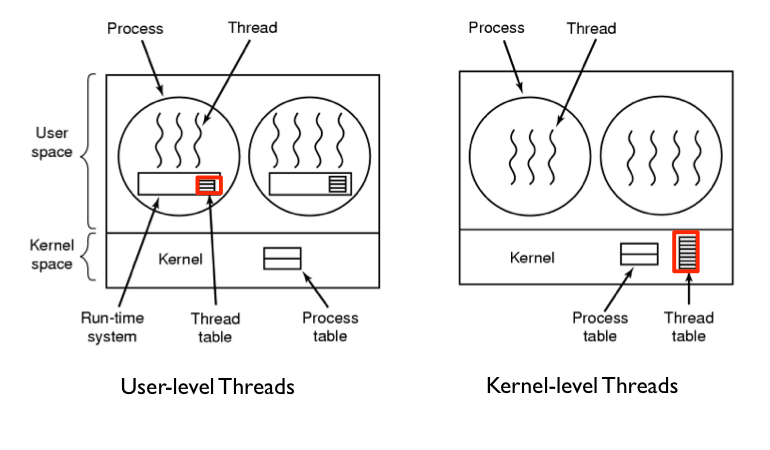
\includegraphics[scale=.43]{usr-vs-kernel.png}
\begin{itemize}
  \item {\bf User Lever}
    \begin{itemize}
      \item \underline{Advantages}
        \begin{itemize}
          \item Fast Context Switching: keep the OS out of it!
          \begin{itemize}
            \item User level thread libraries do not require system calls
            \item Have to use thread-yield:
                \item save the thread information into the thread table
                \item Call the thread scheduler to pick another thread to run
            \item Saving local thread state scheduling are local procedures
            \item Customized scheduling
          \end{itemize}
        \end{itemize}
      \item \underline{Disadvantages}
        \begin{itemize}
          \item What happens if one thread makes a blocking I/O call?
            \begin{itemize}
              \item Change the system to be non-blocking
              \item Always check to see if a syscall will block
            \end{itemize}
          \item What happens if one thread never yields?
            \begin{itemize}
              \item Introduce clocked interrupts
            \end{itemize}
          \item Multi-threaded programs frequently make system calls
            \begin{itemize}
              \item Causes a trap into the kernel anyway!
            \end{itemize}
        \end{itemize}
    \end{itemize}
  \item {\bf Kernel-level Threads}
  \begin{itemize}
    \item \underline{Advantages}
      \begin{itemize}
        \item Kernel schedules threads in addition to processes
        \item Multiple threads of a process can run simultaneously
          \begin{itemize}
            \item Now what happens if one thread blocks on I/O?
            \item Kernel-level threads can make blocking I/O calls w/o blocking other threads of same process
          \end{itemize}
        \item Good for multi core architectures.
      \end{itemize}
    \item \underline{Disadvantages}
      \begin{itemize}
        \item Overhead in the kernel, extra DS, scheduling\dots
        \item Thread creation is expensive.
        \item Which thread should receive a signal?
      \end{itemize}
  \end{itemize}
\end{itemize}
% subsection What are the advantages and disadvantages of kernel-level threads over user-level threads? (end)
\subsection{Compare the use of fork() to the use of pthread-create()} % (fold)
\label{sub:Compare the use of fork() to the use of pthread_create()}
pthread-create() creates a thread. The thread will start from the function that is passed withing the argument. Instead, fork will create a process, which will start from the next line, and return 0 to the child pid.
% subsection Compare the use of fork() to the use of pthread-create() (end)
\subsection{In a multiprocessor system, what conditions will cause threads within a process to block?} % (fold)
\label{sub:In a multiprocessor system, what conditions will cause threads within a process to block?}
\begin{itemize}
  \item Blocking call to I/O.
  \item Waiting for other threads.
  \item Shared memory might cause a block as well
\end{itemize}
% subsection In a multiprocessor system, what conditions will cause threads within a process to block? (end)
\subsection{Explain how a process can become orphaned and what the OS does with it. How about zombies?} % (fold)
\label{sub:Explain how a process can become orphaned and what the OS does with it. How about zombies?}
A process becomes orphan when his parent is killed, via a SEGFAULT or exit call. In case of an error, the OS is going to kill it.
Otherwise, the process is going to keep running normally. A zombie is going to get killed by the OS whenever the parent
is going to terminate.
% subsection Explain how a process can become orphaned and what the OS does with it. How about zombies? (end)
\subsection{Describe how to use the POSIX call wait()} % (fold)
\label{sub:Describe how to use the POSIX call wait()}
POSIX wait call is made for processes. It makes a parent process wait until its child process terminates. Useful for several reasons. Also, by waiting, the parent will make reap on his child, destroying all the traces of that process.
% subsection Describe how to use the POSIX call wait() (end)
\subsection{Explain what happens when a process calls exec()} % (fold)
\label{sub:Explain what happens when a process calls exec()}
\begin{itemize}
  \item Load and runs in current process:
    \begin{itemize}
      \item Executable filename
      \item With argument list argv
      \item And environment variable list envp
    \end{itemize}
  \item Does not return( unless error)
  \item Overwrites code, data, and stack
  \begin{itemize}
    \item Keeps PID, open files and signal context.
  \end{itemize}
\end{itemize}
% subsection Explain what happens when a process calls exec() (end)
\subsection{Explain how re-entrant functions are used in C.} % (fold)
\label{sub:Explain how re-entrant functinos are used in C.}
A re-entrant function is one that can be interrupted in the middle of its execution and then safely called again before its previous invocations complete executing. They are used if you have code that will have HW interrupt or signal. They are so called
thread safe functions.
% subsection Explain how re-entrant functions are used in C. (end)
\subsection{What are the maximum number of threads that can be run concurrently?} % (fold)
\label{sub:What are hte maxium number of threads that can be run concurrently?}
It depends by the number of cores on your machine.
% subsection What are the maximum number of threads that can be run concurrently? (end)
\subsection{If a process spawns a number of threads, in what order will these threads run?} % (fold)
\label{sub:If a process spawns a number of threads, in what order will these threads run?}
There is no way of knowing. It depends by the scheduling of the system, in case of kernel-threads. If you are implementing
user threads, then you might be able to know.
% subsection If a process spawns a number of threads, in what order will these threads run? (end)
\subsection{Explain how to use pthread-detach() and pthread-join() and why these are used.} % (fold)
\label{sub:Explain how to use pthread-detach() and pthread-join() and why these are used.}
detach() is used if you have a joinable thread and you want to make it detachable. Then, ti meas you do not care anymore about
that thread to return, and you will not wait anymore for it. \\
join() instead is used to make a thread wait for other threads, if they were specified to be joinable. Then, you will get
the return value of the other thread, and you will be able to know when its going to return.
% subsection Explain how to use pthread-detach() and pthread-join() and why these are used. (end)
\subsection{Explain how a shell process can execute a different program} % (fold)
\label{sub:Explain how a shell process can execute a different program}
It can do so by using fork(), followed by execve. Here is an example:
\begin{lstlisting}
 
  /* start fork */
  pid_t pid = fork();
  int child_status;

  if ( pid == 0 ) // child
  {
    int ret = execvp(arg1, cmd);
    if ( ret < 1 ) puts ("the comand does not exits");
    _exit(0);
  }
  else if ( pid < 0 )
  {
    puts("Failed to fork");
    exit(1);
  }
  else // parent
    wait( & child_status);
\end{lstlisting}

% subsection Explain how a shell process can execute a different program (end)
\subsection{Explain how one process can wait on the return value of another process} % (fold)
\label{sub:Explain how one process can wait on the return value of anotehr process}
By using wait() look at the example above.
% subsection Explain how one process can wait on the return value of another process (end)
\subsection{Describe the transitions between running, ready and blocked in the 5 state model.} % (fold)
\label{sub:Describe the transitions between running, ready and blocked in the 5 state model.}
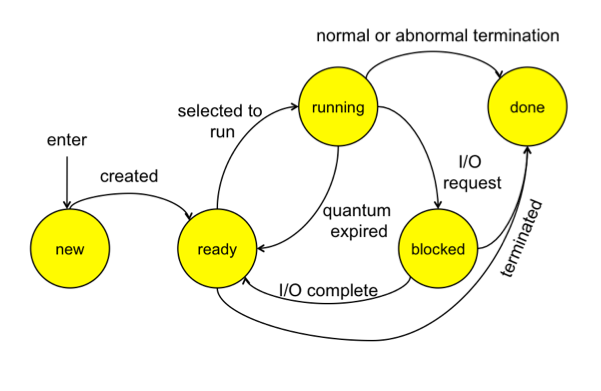
\includegraphics[scale=.60]{5-state-trans.png}
% subsection Describe the transitions between running, ready and blocked in the 5 state model. (end)
% section Thread and Processes (end)
\section{Scheduling} % (fold)
\label{sec:Scheduling}
{\bf High-level objectives} \\
\begin{tabular}{| c | l |}
  \hline
  {\bf Objective} & \\
  \hline
  Fairness & Equitable share of resources \\
  Priority & Allocate to most important first \\
  Efficiency & Make best use of equipment \\ 
  Encourage good behavior & Can't take advantage of the system \\
  Support heavy loads & Degrade gracefully \\
  Adapting to different environments & interactive, real-time, multi-media  \\
  \hline
\end{tabular}
\\
{\bf Quantitative objectives} \\
\begin{tabular}{| c | l |}
  \hline
  {\bf Objective} & \\
  \hline
  Fairness & Processes get close to equal share of the CPU \\
  Efficiency & Keep resources as busy as possible \\
  Throughput & Number of processes that complete per unit time \\
  Waiting time & Time a process spends waiting in kernel's ready queue \\
  Turnaround time & time from process start to its completion \\
  Response time & Amount of time from when a request was first \\
                & submitted until first response is produced \\
  \hline
\end{tabular}


\subsection{Which policies have the possibility of resulting in the starvation of processes?} % (fold)
\label{sub:Which policies have the possibility of resulting in the starvation of processes?}
Shortest job first and priority based algorithms can result in starvation of the process. The reason why is that you risk of 
always having other processes coming before, cutting the running time of the processes.
% subsection Which policies have the possibility of resulting in the starvation of processes? (end)
\subsection{Which scheduling algorithm results results in the smallest AWT?} % (fold)
\label{sub:Which scheduling algorithm results results in the smallest AWT?}
Preemptive SJF has provably the best AWT. in fact, in PSJF, the shortest processes always preempt the longer ones, minimizing
the waiting time.
% subsection Which scheduling algorithm results results in the smallest AWT? (end)
\subsection{What scheduling algorithm has the longest average response time?} % (fold)
\label{sub:What scheduling algorithm has the longest average response time?}

% subsection What scheduling algorithm has the longest average response time? (end)
\subsection{Define turnaround time, waiting time and response time in the context of scheduling algorithms} % (fold)
\label{sub:Define turnaround time, waiting time and response time in the context of scheduling algorithms}

% subsection Define turnaround time, waiting time and response time in the context of scheduling algorithms (end)
\subsection{What is the Convoy Effect?} % (fold)
\label{sub:What is the Convoy Effect?}
Is when all I/O processes are waiting for a long CPU process or vice versa. Thus, not smart utilization of resources. \\
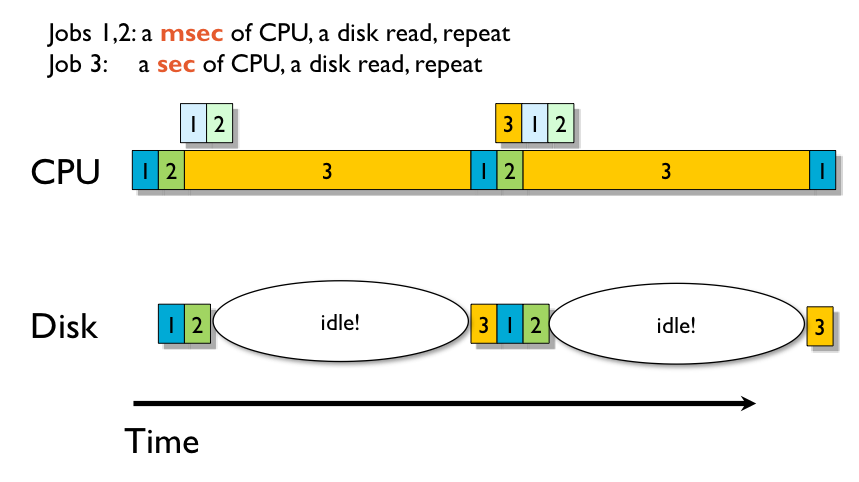
\includegraphics[scale=.45]{convoy.png}
% subsection What is the Convoy Effect? (end)
\subsection{Why do processes need to be scheduled?} % (fold)
\label{sub:Why do processes need to be scheduled?}
Scheduling is deciding which process/thread should occupy each resource at each moment. We need it because when we have a pool
of processes to choose from in ready state, we need to make a decision on which process is going to run, for how long and with
what resource
% subsection Why do processes need to be scheduled? (end)
\subsection{What is starvation?} % (fold)
\label{sub:What is starvation?}
It means that the longest or low priority jobs may never be ended up scheduling, as the scheduler never pick them.
% subsection What is starvation? (end)
\subsection{What is response time? what other metrics do we use to evaluate scheduling algorithms} % (fold)
\label{sub:What is response time? what other metrics do we use to evaluate scheduling algorithms?}
\begin{itemize}
  \item {\bf Response time}
    \begin{itemize}
      \item Amount of time from when a request was first submitted until first response is produced
    \end{itemize}
  \item {\bf Throughput}
    \begin{itemize}
      \item Number of processes that complete per unit time
    \end{itemize}
  \item {\bf Waiting time}
    \begin{itemize}
      \item Time a process spends waiting in kernel's ready queue
    \end{itemize}
  \item {\bf Turnaround time}
    \begin{itemize}
      \item Time from process start to its completion
    \end{itemize}
\end{itemize}
% subsection What is response time? what other metrics do we use to evaluate scheduling algorithms? (end)
\subsection{Which scheduling algorithm minimizes avg initial response time? Waiting time? Turnaround time?} % (fold)
\label{sub:Which scheduling algorithm minimizes avg intitial response time? Waiting time? Turnaround time?}
\begin{itemize}
  \item {\bf Initial response time}
    \begin{itemize}
      \item Round-robin, as every process will get scheduled in an average time quantum.
    \end{itemize}
  \item {\bf Waiting time}
    \begin{itemize}
      \item Shortest Job First has provably the best waiting time.
    \end{itemize}
  \item {\bf Turnaround time}
    \begin{itemize}
      \item Probably, SJF and Round robin.
    \end{itemize}
\end{itemize}
This table reassures all the qualities. \\
\begin{tabular}{| c | c | l | l | r |}
  \hline
  {\bf Scheduling algorithm} & {\bf CPU overhead} & {\bf Throughput} & {\bf Turnaround time} & {\bf Response time} \\
  \hline
  {\bf First in First out} & Low            & Low              & High                  & Low \\
  \hline
  {\bf Shortest Job First} & Medium            & High              & Medium                  & Medium \\
  \hline
  \hline
  {\bf Priority based} & Medium            & Low              & High                  & High \\
  \hline
  {\bf Round-Robin} & High            & Medium              & Medium                  & High \\
  \hline
  {\bf Multilevel Queue} & High            & High              & Medium                  & Medium \\
  \hline
\end{tabular}
% subsection Which scheduling algorithm minimizes avg initial response time? Waiting time? Turnaround time? (end)
\subsection{Why are SJF and Preemptive SJF hard to implement in real systems?} % (fold)
\label{sub:Why are SJF and Preemptive SJF hard to implement in real systems?}
Because you are required to know the running time of the process, which is impossible because of the Halting problem.
Systems that implement this type of scheduling look at 
% subsection Why are SJF and Preemptive SJF hard to implement in real systems? (end)
\subsection{What does it mean to preempt a process?} % (fold)
\label{sub:What does it mean to preempt a process?}
It is the act of temporarily interrupting a task, without requiring its cooperation, with the intention of resuming the task at a later time. Such a change is called context switch.
% subsection What does it mean to preempt a process? (end)
\subsection{What does it mean for a scheduling algorithm to be preemptive?} % (fold)
\label{sub:What does it mean for a scheduling algorithm to be preemptive?}
It means that it will block a thread after a fixed time quantum expires. This is done to ensure that no process will suffer of
starvation.
% subsection What does it mean for a scheduling algorithm to be preemptive? (end)
\subsection{Describe the Round-Robin scheduling algorithm. Explain the performance advantages and disadvantages} % (fold)
\label{sub:Describe the Round-Robin scheduling algorithm. Explain the performance advantages and disadvantages}
{\bf Round Robin} 
Select process/thread from ready queue in a round-robin fashion. \\
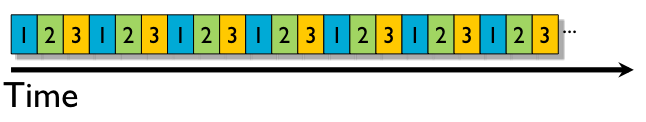
\includegraphics[scale=.45]{roundrobin.png}
\begin{itemize}
  \item {\bf Advantages}
    \begin{itemize}
      \item Jobs get fair share of CPU
      \item Shortest jobs finish relatively quickly
    \end{itemize}
  \item {\bf Disadvantages}
    \begin{itemize}
      \item Might want some jobs to have greater share
      \item Context switch overhead
      \item Poor average waiting time with similar job lengths
      \item Performance depends on length of time quantum
    \end{itemize}
\end{itemize}
% subsection Describe the Round-Robin scheduling algorithm. Explain the performance advantages and disadvantages (end)
\subsection{Describe the First Come First Serve (FCFS) scheduling algorithm. Explain the performance advantages and disadvantages.} % (fold)
\label{sub:Describe the First Come First Serve (FCFS) scheduling algorithm. Explain the performance advantages and disadvantages.}
\begin{itemize}
  \item Process that requests the CPU first is allocated the CPU first
  \item Non-preemptive
  \item Implementation
    \begin{itemize}
      \item FIFO queues
      \item A new process enters the tail of the queue
      \item The scheduler selects next process to run from the head of the queue
    \end{itemize}
  \item {\bf Advantages:}
    \begin{itemize}
      \item Simple implementation.
      \item Good for some specific implementation
    \end{itemize}
  \item {\bf Problems: }
    \begin{itemize}
      \item Non-preemptive
      \item Non optimal AWT
      \item Cannot utilize resources in parallel
      \item Result:
        \begin{itemize}
          \item Waiting time depends on arrival order
          \item Potentially long wait for jobs that arrive later
          \item Convoy effect, low CPU and I/O device utilization
        \end{itemize}
    \end{itemize}
\end{itemize}
% subsection Describe the First Come First Serve (FCFS) scheduling algorithm. Explain the performance advantages and disadvantagessubsection name. (end)
\subsection{Describe the Pre-emptive and Non-preemptive SJF scheduling algorithms. Explain the performance advantages and disadvantages} % (fold)
\label{sub:Describe the Pre-emptive and Non-preemptive SJF scheduling algorithms. Explain the performance advantages and disadvantages}
\begin{itemize}
  \item Job with shortest CPU time goes first
    \begin{itemize}
      \item Often used in batch systems
    \end{itemize}
  \item it is either preemptive or non-preemptive
  \item \underline{Non preemptive}
    \begin{itemize}
      \item {\bf Advantages}
        \begin{itemize}
          \item Low average waiting time
          \item Helps keep I/O devices busy
        \end{itemize}
      \item {\bf Disadvantages}
        \begin{itemize}
          \item Not practical: cannot predict future CPU burst time
          \item Starvation: Long jobs may never be scheduled.
        \end{itemize}
    \end{itemize}
  \item \underline{ Preemptive SJF}
    \begin{itemize}
      \item Algorithm
        \begin{itemize}
          \item Job with least remaining time to completion runs
          \item So, a new job that is shorter than remainder of running job preempts it
        \end{itemize}
      \item {\bf Advantages}
        \begin{itemize}
          \item Similar to non-preemptive SJF
          \item Provably minimal average waiting time
        \end{itemize}
      \item {\bf Disadvantages}
        \begin{itemize}
          \item Starvations again: long job keeps getting preempted by shorter ones.
        \end{itemize}
    \end{itemize}
\end{itemize}
% subsection Describe the Pre-emptive and Non-preemptive SJF scheduling algorithms. Explain the performance advantages and disadvantages (end)
\subsection{Describe the Preemptive Priority-based scheduling algorithm. Explain the performance advantages and disadvantages.} % (fold)
\label{sub:Describe the Preemptive Priority-based scheduling algorithm. Explain the performance advantages and disadvantages.}
\begin{itemize}
  \item Rationale
    \begin{itemize}
      \item Higher priority jobs are more mission-critical
    \end{itemize}
  \item Each job is assigned a priority
  \item Select highest priority runnable job
    \begin{itemize}
      \item FCFS or Round Robin to break ties
    \end{itemize}
  \item {\bf Disadvantages}
    \begin{itemize}
      \item May not give the best AWT
      \item Starvation of lower priority processes.
    \end{itemize}
\end{itemize}
% subsection Describe the Preemptive Priority-based scheduling algorithm. Explain the performance advantages and disadvantages. (end)
\subsection{How does the length of the time quantum affect Round-Robin scheduling?} % (fold)
\label{sub:How does the length of the time quantum affect Round-Robin scheduling?}
It changes a lot regarding the performance of your scheduler, as changes AWT, number of context switches and much more.
\begin{itemize}
  \item Choice depends on
    \begin{itemize}
      \item Priorities, architecture
    \end{itemize}
  \item Typical quantum: 10-100 ms
    \begin{itemize}
      \item Large enough that overhead is small percentage
      \item Small enough to give illusion of concurrency
    \end{itemize}
\end{itemize}
% subsection How does the length of the time quantum affect Round-Robin scheduling? (end)
\subsection{Define fairness in terms of scheduling algorithms. What are the fairness properties of each of the scheduling disciplines discussed in class?} % (fold)
\label{sub:Define fairness in terms of scheduling algorithms. What are hte fairness properties of each of hte scheduling disciplines discussed in class?}
By fairness, we mean that each process gets an equitable share of resources. In a more quantitative lever, we mean that the processes
get close to an equal share of the CPU.
% subsection Define fairness in terms of scheduling algorithms. What are the fairness properties of each of the scheduling disciplines discussed in class? (end)
\subsection{Which scheduling algorithms guarantee progress?} % (fold)
\label{sub:Which scheduling algorithms guarantee progress?}
Round Robin, First Comes First Serves are guaranteed to never make your process starve.
% subsection Which scheduling algorithms guarantee progress? (end)
\subsection{A process was switched from running to ready state. Describe hte characteristics of the scheduling algorithm being used} % (fold)
\label{sub:A process was switrhed from running to ready state. Describe hte characteristics of the scheduling algorithm being used}
The process must be preemptive. In fact, if such a transition happens, it implies that the job must have ran out of its time quantum.
% subsection A process was switched from running to ready state. Describe hte characteristics of the scheduling algorithm being used (end)
% section Scheduling (end)
% =========================================================

\section{Synchronization} % (fold)
\label{sec:Synchronizatio}
\begin{enumerate}
  \item	{\bf What is the readers-writers problem? } \\
    It is a generalization of the mutual exclusion problem. You have \emph{ readers} which can only read the object, \emph{ writer} threads that can only modify the thread. This problem occurs frequently in real time systems.

  \item {\bf  What is the producers-consumers problem? } \\
    You have some consumer and some producers, which share a buffer. The point is if the buffer is full, then producers must wait. Else, if buffer is empty, consumers must wait. So, the point is to find a balance in between.

  \item {\bf  What is the dining philosopher problem? } \\
   You have $n$ dining philosophers, and only $n$ forks. Each philosopher needs two forks to eat. The point of the problem is to have them eat without encounter a deadlock. 

 \item {\bf  Recognize a correct solution to the readers-writers problem, the producers-consumers problem, and the dining philosopher.  Be able to identify and explain an error in a specific implementation of any of the classic synchronization problems. } \\
    \begin{itemize}
      \item {\bf Readers-writers: } \\
        use conditional variable to signal whether its safe or not. Otherwise, just wait for your turn.
      \item {\bf Producer- consumer:} \\ 
        You can use a mutex to signal the shared buffer, thus insert or remove item, and a semaphore to signal the number of empty slots, as well as the number of filled slots.
      \item {\bf Dining philosophers:} \\
        You can make the philosophers request resources in order. This way, you will be guaranteed to be able to always avoid deadlocks.
    \end{itemize}

  \item {\bf  What happens when readers are prioritized over writers in the classic “readers writer problem”?  How about if writers are prioritized over readers?} \\
    \begin{itemize}
      \item \underline{Favor readers:} No reader waits unless a writer is already in critical section. A reader that arrives after a waiting writer gets priority over a writer.
      \item \underline{Favor writers:} Once a writer is ready to write, it performs its write as soon as possible. A reader that arrives after a writer must wait, even if the writer is also waiting.
      \item {\bf Both problem suffer of starvation!}
    \end{itemize}

  %%%%% %%%%% %%%%% %%%%% %%%%%
  \item {\bf  What is required so that deadlock and starvation do not occur in the dining philosopher’s problem?  Give examples of solutions. }\\

    \begin{itemize}
      \item You can make the philosophers request resources in order. This way, you will be guaranteed to be able to always avoid deadlocks.
      \item No hold and wait: do not allow the philosophers to hold the resources while waiting.
    \end{itemize}

  %%%%% %%%%% %%%%% %%%%% %%%%%
  \item {\bf  What is the difference between starvation, deadlock, race conditions and critical sections?  Describe each. } \\
    \begin{itemize}
      \item \underline{Starvation:} A thread is always waiting for some other event to finish.
      \item \underline{Deadlock:} Each process is waiting for another one in a circular manner
      \item \underline{Race conditions:} Occurs when separate processes or threads of execution depend on some shared state.
      \item \underline{Critical sections:} Operations upon shared states. They must be ensured to be mutual exclusive for the system to work correctly.
    \end{itemize}

  %%%%% %%%%% %%%%% %%%%% %%%%%
  \item {\bf  What would happen if a system’s hardware synchronization primitive were replaced with a software function? } \\
    I guess it would still work. Nevertheless, you could not achieve the same performances as in with hardware, and you would lack security features that hardware provides.

  %%%%% %%%%% %%%%% %%%%% %%%%%
  \item {\bf  Which type of variables must be protected against concurrent readers and writers in any combination?} \\
    Shared variables. That is, variables on the heap or global status variables.

\end{enumerate}
% section Synchronizatio (end)

\section{Semaphores / Mutexes} % (fold)
\label{sec:Semaphores / Mutexes}
\subsection{Semaphores for mutual exclusion} % (fold)
\label{sub:Semaphores for mutual exclusion}
Some terminology:
\begin{itemize}
  \item {\bf Binary semaphore}
    \begin{itemize}
      \item Semaphore whose value is always 0 or 1
    \end{itemize}
  \item {\bf Mutex }
    \begin{itemize}
      \item binary semaphore used for mutual exclusion
      \item Used for exclusive access to a shared resource (critical section)
        \begin{itemize}
          \item \emph{wait} operation: ``locking'' the mutex
          \item \emph{post} operation: ``unlocking'' or ``releasing'' the mutex
          \item \emph{Holding} a mutex: locked and not yet unlocked
        \end{itemize}
    \end{itemize}
  \item {\bf Semaphore}
    \begin{itemize}
      \item Generalization of mutexes: count nubmer of available ``resources''
      \item Wait for an available resource (--), notify availability (++)
      \item Example: wait for free buffer spae, signal more buffer space
    \end{itemize}
  \item {\bf Condition variables}
    \begin{itemize}
      \item Represent an arbitrary event
      \item Operations: wait foe even, signal occurrence of event 
      \item Tied to a mutex for mutual exclusion
    \end{itemize}
\end{itemize}
{\bf Semaphores vs. condition variables} \\
\begin{tabular}{| c | c |}
  \hline
 {\bf Semaphore} & {\bf Condition Variable} \\
  \hline
 Integer value $(\geq 0)$ & No integer value \\
  \hline
 Wait doesn't always block & Wait always blocks \\
  \hline
 Signal either un-blocks thread || increments counter & Signal either un-block thread or is lost \\
  \hline
 if signal releases thread, both may continue concurrently & if signal releases thread, only one continues\\
  \hline
\end{tabular}
% subsection Semaphores for mutual exclusion (end)
\subsection{When do you have to use a semaphore or mutex?} % (fold)
\label{sub:When do you have to use a semaphore or mutex?}
When memory does not have a single clear cut owner, or when the two threads need to work together. In this cases, you cannot have
separate memory, therefore you need a way of synchronizing the work of the two thread.
% subsection When do you have to use a semaphore or mutex? (end)
\subsection{What is mutual exclusion?} % (fold)
\label{sub:What is mutual exclusion?}
Mutual exclusion refers to the problem of ensuring that no two processes or threads can be in their critical section at the same time. 
% subsection What is mutual exclusion? (end)
\subsection{How can you use a mutex lock to ensure that concurrent code operates correctly?} % (fold)
\label{sub:How can you use a mutex lock to ensure that concurrent code operates correctly?`}

\begin{lstlisting}
  #include<semaphore.h>
  ...
  int cnt=0;
  sem_t cnt_mutex;

  int main(void)
  {
    ...
    /* initialize mutex */
    result = sem_init( & cnt_mutex, 0, 1);
    if ( result < 0)
      exit(-1);
    ...

    /* Clean up the semaphore that we're done with */
    result = sem_destroy( & cnt_mutex);
    assert( result == 0 ); 
  }

  void * worker ( coid * ptr)
  {
    int i;
    for ( i=0; i < ITERATIONS_PER_THREAD;i ++) {
      sem_wait( & cnt_mutex);
      cnt++;
      sem_post( & cnt_mutex);
      }
  }
\end{lstlisting}
% subsection How can you use a mutex lock to ensure that concurrent code operates correctly? (end)


\begin{enumerate}
  \item {\bf Understand the common semaphore and mutex functions (sem\_wait(), sem\_post(), etc). } \\
    \begin{itemize}
      \item \underline{*\_wait()}: you ask you semaphore to wait until post operation, which is exit from the critical section. It locks the mutex.
      \item \underline{*\_post():} you increment the mutex, thus you release it from the blocked state.
    \end{itemize}

  \item {\bf What are proper and improper code replacements for a test\_and\_set() operation? } \\
    you have to use atomic wait and post operations. This is an example:
    \begin{lstlisting}
      boolean test_and_set(boolean* lock) atomic {
        boolean initial = *lock;
        *lock = true;
        return initial;
      }
    \end{lstlisting}

  \item {\bf How does the internal counter of a POSIX semaphore work?  What does it mean if the value of the semaphore is 1?}\\
    If the value of a semaphore is $1$, then we will keep waiting, as we are stuck in a while(1) loop.

  \item {\bf How can the reader-writer problem be solved using only POSIX mutexes? }\\
    You can make either writer or reader wait until a certain condition.
  \item {\bf Using only one mutex, is it possible to create a semaphore?  If so, how?  If not, why?} \\
    Yes, you can. You can associate a counter with that mutex, thus creating a semaphore. Though, you have to make sure that your mutex will not always block and that your counter has mutual exclusion.

  \item {\bf What are condition variables?  Understand how they can be used in code. } \\
    Conditional variables represent an arbitrary event. The operations are wait for event, signal occurrence of event. It is strictly tied to a mutex for mutual exclusion.
\end{enumerate}
% section Semaphores / Mutexes (end)
\section{Processes and Deadlock} % (fold)
\label{sec:Processes and Deadlock}
\begin{enumerate}
  \item {\bf Define deadlock. }\\
    There exists a cycle of processes such that each process cannot proceed until the next process takes some specific action.

  %%%%% %%%%% %%%%% %%%%% %%%%%
  \item {\bf Define circular wait, mutual exclusion, hold and wait, and no preemption. How are these related to deadlock? }\\
    \begin{itemize}
      \item \underline{Circular wait:} Every process is waiting for another in a circle fashion. Look definition of deadlock. 
      \item \underline{Mutual exclusion:} Shared memory that two threads cannot access at the same time. Deadlocks work on mutual exclusion.
      \item \underline{Hold and wait:} A thread gets right on an object and keeps waiting to have other right to get the rest of work. Can cause a deadlock.
      \item \underline{No preemption:} A system will not stop a process from running. With preemptive, you will automatically resolve deadlocks, as you are giving up resources. 
    \end{itemize}

  %%%%% %%%%% %%%%% %%%%% %%%%%
  \item {\bf How would the implementation of a web server using threads differ from one using processes? }\\
    It is a lot faster. You really do not need to run a process per incoming connection. However, you might have slight more complications due to the fact that you will need some good semaphores ad mutexes.

  %%%%% %%%%% %%%%% %%%%% %%%%%
  \item {\bf What can happen if synchronization in a multiple-threaded program is not programmed carefully? } \\
    Race conditions will be broken. Everything could happen, is a free for all. Wrong data, segfauls, broken process flow$\dots$. Anything really.

  %%%%% %%%%% %%%%% %%%%% %%%%%
  \item {\bf Why might an operating system use a resource allocation graph? } \\
    Because you will eb able to see which process allocated what, thus ensure to keep mutual exclusion.

  %%%%% %%%%% %%%%% %%%%% %%%%%
  \item {\bf What are the conditions of a deadlock? How could you guarantee that each one of these conditions can be prevented? }\\
    \begin{itemize}
      \item Mutual exclusion: give non-exclusive access only, read-only access.
      \item hold-and-wait: Make a process request all the resources at one time. 
      \item No preemption condition: Allow preemption! It will break circular wait now.
      \item Circular wait condition: Number resources and make processes ask for the minimum resource.
    \end{itemize}

    %%%%% %%%%% %%%%% %%%%% %%%%%
    \item {\bf What does waitpid() do? } \\
      Makes a process wait for another one, and then rips it whenever it finishes.

  %%%%% %%%%% %%%%% %%%%% %%%%%
  \item {\bf What is the difference between Deadlock Prevention, Deadlock Detection \& Recovery, and Deadlock Avoidance? What deadlock handling mechanism would you use? } \\
    \begin{itemize}
      \item \underline{Prevention:} Design system so that deadlock is impossible
      \item \underline{Avoidance:} Steer around deadlock with smart scheduling
      \item \underline{Detection \& recovery:} Check for deadlock periodically, recover by killing a deadlocked processes and releasing its resources. 
    \end{itemize}
    The mechanism very much depends on what your goals are. If they are rare, and not worth the overhead, then even none of them.

  %%%%% %%%%% %%%%% %%%%% %%%%%
  \item {\bf What are the components of a resource allocation graph?}\\
    Process, resource, request, ownership.

  %%%%% %%%%% %%%%% %%%%% %%%%%
  \item {\bf What problem does the Banker’s Algorithm solve? Given a set of processes how would you use the Banker’s Algorithm? }\\
    Thanks to the banker algorithm, we are able to check if a given state of a system is safe. The steps are:\\
    Upon a resource allocation request:
    \begin{enumerate}
      \item Pretend that we approve the request.
      \item Call function: would we then be safe?
      \item If save, then \underline{approve}. Else, \underline{reject}.
    \end{enumerate}

  %%%%% %%%%% %%%%% %%%%% %%%%%
  \item {\bf What is a safe state and how can you determine if a system is in a safe state? } \\
    There exists and execution order that can finish. In general, its hard to predict. Can do so by trying out.
\end{enumerate}
% section Processes and Deadlock (end)
\section{Interprocess communication} % (fold)
\label{sec:Interprocess communicatio}
\begin{enumerate}
  \item {\bf What is the difference between a FIFO and a pipe?}\\
    FIFOs are named pipes. They are special pipes that persist even after all the processes have closed them. They are actually implemented as a file. Memory persists.

  \item {\bf How would you redirect standard out to a file? }\\
    \begin{lstlisting}
    int bak, new;
    fflush(stdout);
    bak = dup(1);
    new = open("/dev/null", O_WRONLY);
    dup2(new, 1);
    close(new);
    /* your code here ... */
    fflush(stdout);
    dup2(bak, 1);
    close(bak);
    \end{lstlisting}

  \item {\bf What happens when two processes read and write to a memory mapped file?} \\
    If its shared memory, then the mutual exclusion must be provided by the user. Otherwise the mutual excursion is provided by the OS.

  \item {\bf Explain how two processes can share memory using shmem. } \\
    \begin{enumerate}
      \item Create identifier (``key'') for a shared memory segment.
        \begin{lstlisting}
        key_t ftok(const char *pathname, int proj_id);
        k = ftok(“/my/file”, 0xaa);    
        \end{lstlisting}
      \item Create shared memory segment
        \begin{lstlisting}
        int shmget( key_+t key, size_t size, int shmflg);
        id = shmget(key, size, 0644 | IPC_CREAT);
        \end{lstlisting}
      \item Access to shared memory requires an attach
        \begin{lstlisting}
        void *shmat(int shmid, const void *shmaddr, int shmflg);
        shared_memory = (char *) shmat(id, (void *) 0, 0); 
        \end{lstlisting}
    \end{enumerate}

  \item {\bf Explain how a process can set which signals are caught or ignored using a signal set. } \\
    Using a custom signal handler. Any process can modify its signal handler simply by changing the signal mask of the given process, and specifying a new handler function. Here is an example:
    \begin{lstlisting}
      struct sigaction sa;
      sa.sa_handler = handle;  /* the handler function!! */
      sa.sa_flags = 0;
      sigemptyset(&sa.sa_mask);

      sigaction(SIGING, &sa, NULL);
    \end{lstlisting}

  \item {\bf How can one process send a signal to another?} \\
    Using the simple syscall \underline{kill(pid,signal)}. Works like in the shell.

  \item {\bf Describe the purpose of a POSIX signal. } \\
    Communicating between processes, invalid memory accesses, program termination\dots. anything that involves certain specific actions.
  \item {\bf Some signals cannot caught or ignored. Which signals are they and why shouldn’t they be allowed to be caught? }\\
    SIGSEGV should not be ignored, as well as SIGKILL and SIGALRM.

  \item {\bf What does “kill -<parameter> pid” do?} \\
    Sends signal number <parameter> to the given pid.

  \item {\bf How is the function sigwait() used?} \\
    the \emph{sigwait()} function shall select a pending signal from set, atomically clear it from the system's set of pending signals, and return that signal number in the location referenced by sig.

  \item {\bf How does the function alarm() work?} \\
    Sends a SIGALRM after the time specified in the parameter.
\end{enumerate}
% section Interprocess communicatio (end)
\section{Networking} % (fold)
\label{sec:Networking}
\begin{enumerate}
  \item {\bf When do you use the close() system call with sockets? } \\
    You use close when you want to tear down a connection on both side. After it, you cannot write again to that socket.

  \item {\bf Discuss how a multithreaded web server running on a single processor system could be optimized using the process scheduling methods discussed in class. Which do you recommend? }\\
    I would probably use a round robin. In fact, By using RR you ensure that every client gets a fair share of the server, and most important, that everybody gets an answer in a quick time.

  \item {\bf How do select() and poll() work? What problem do they it solve? } \\
    You use them to wait for input. Select waits for readable/ writable file descriptors, whereas polls quereis the file descriptors for  the events that you are asking.

  \item {\bf Describe the Posix accept() function. } \\
    Accept blocks waiting for a new connection. It returns the value of a socket description that the connection will be moved, so that you can still communicate over the previous socket.

  \item {\bf How does HTTP work? } \\
    The Hypertext Transfer Protocol is a communication protocol between client/server. It uses TCP and the purpose is transferring files and stuff. You can transfer a single or multiple file at once  depending on the type of connection requested.

  \item {\bf Describe the services provided by TCP.} \\
    TCP provides reliable connection oriented transmission. It provides reliable transport, flow control and congestion control. However, it does not provide timing, throughput guarantees and security.
    
  \item {\bf How does TCP connection establishment work? }\\
    You need to cave a TCP connection request, and a TCP connection response. That happens through the SYN packet.

  \item {\bf Describe the services provided by UDP.} \\
    Provides unreliable data transfer. Does not provide: connection setup, reliability, flow control, congestion control, timing, throughput guarantee or security.

  \item {\bf How do sockets support the client-server model? }\\
    We use two ways to initialize a socket. The first one, the server listen for an incoming connection, in a so called ``server socket''. Then, the client connects to the socket and the server accepts the incoming connection.

  \item {\bf Which is better, UDP or TCP? Which one would you use?} \\
    I would use TCP. In fact, it would provide me with a reliable connection and a higher lever service.

  \item {\bf How does the Domain Name System (DNS) work? }\\
    The DNS system is a layer of indirecting between the IP address and the browser. It requests a recursive query of the different domains of several layers.
  \item {\bf How does DNS use caching?} \\
    You use caching as it greatly improves the time of response. Therefore, you have a caching local server to answer all the local requests, so that you don't have to go query the foreign server.

  \item {\bf How is DNS related to IP? }\\
    DNS translate into IP addresses.
\end{enumerate}
% section Networking (end)
\section{File system and I/O} % (fold)
\label{sec:File system and I/O}
\begin{enumerate}
  \item {\bf Given a description of the block size and i-node structure, what is the maximum size of a file? } \\
    block size * inode\_num + offset
  \item {\bf How many i-node operations are required to fetch a file at /path/to/file? }\\
    The number of directories from the root to the file. 

  \item {\bf What information is stored in an i-node?  What information isn’t? } \\
    The inode number  is just the ``index'' of the inode, so that you can go and access the rest of the system from your disk. Also, an inode stores all the information about a regular file, directory or other file system, except its data and name. That is:
    \begin{itemize}
      \item Size of the file in bytes.
      \item Device ID (this identifies the device containing the file).
      \item The Used ID of the file's owner.
      \item The Group ID of the file.
      \item The file mode which determines the file type and how the file's owner, its group, and others can access the file.
      \item Link count telling how many hard links point to the idone.
      \item Timestamps for may different things.
    \end{itemize}

  \item {\bf What data structure best describes an i-node? } \\
    A bi-directional tree. That is, a tree with nodes going both up and down.

  \item {\bf What are the advantages and disadvantages of an i-node based file system? }\\
    The advantages are that is extensively used in many different places. However, the inode structure presents a simple way and flexible way of using file systems. \\
    There are a number of disadvantages of an extensible inode table. First, the ``negative'' inode space introduces quite a bit of complexity to the inode allocation ad read/write functions. Second, it is not easily extensible to file stems that implement the proposed 64-bit block number extension. Also, it takes aways the beginning portion of the disk.

  \item {\bf Given the description of an i-node file system, how many i-node accesses are required to read the entire contents of a file of a given size?  How many blocks does this file consume on disk? }\\
    it depends on the size of the block and many different things. However, we could derive a simple formula to fet all this values.

  \item {\bf What is an advantage of a soft link over a hard link?} \\
    A soft link does not change the inode structure, bit it binds to the name of another folder. Like that, it is clear what is the target of the node. Instead with a hard link, you don't really know which one is the link and which one is not. Once a soft link gets deleted, only the certain link is deleted. Also, soft links can link to external files or paths that doesn't exist.

  \item {\bf What is I/O polling?  What are advantages and disadvantages?} \\
    In polling, the CPU issues I/O command, writes instructions to the device's registers and waits for completion. However, like this you have a busy waiting, which is the disadvantage, as the CPU always needs to keep polling. Also, it is expensive for large transfers. I is better for small, dedicated systems with infrequent I/O.

  \item {\bf Describe disk I/O access using DMA.}
    Direct memory access is typically done with interrupt-driven I/O. The CPU asks DMA controller to perform device-to-memory transfer. The DMA issues I/O command and transfers new item into memory. The CPU module is interrupted after completion.

  \item {\bf How are file descriptors shared between threads in a single process?  How are they shared between after a process executes a fork()? } \\
    You can share different file descriptors using both caching, and shared memory. 
  
  \item {\bf When the size of a block changes in an i-node based file system, how does this change the maximum size of a file? }\\
    You just need to change the metadata in the files.

  \item {\bf How do polling and interrupt driven I/O differ?  What are the advantages and disadvantages of each? }\\
    \begin{itemize}
      \item \underline{Polling:} Expensive for large transfers. Its better for small, dedicated systems with infrequent I/O.
      \item \underline{Interrupt-driven:} Overcomes CPU busy waiting. I/O module interrupts when ready: event driven. 
    \end{itemize}

  \item {\bf How does the page-out process work? }\\
    You select the pages to evict, those that have not been evicted yet, and then you send them out to disk, so that you have more RAM, which you can use for whatever you need.

  \item {\bf Understand how hard-links result in different file names affecting the same i-node. }\\
    They do so because having multiple links to the same location, it is just like having two paths to the same folder.

  \item {\bf If an i-node based file system has a certain number of direct and single-indirect blocks, how large is the file? }\\
    number of blocks 
  \item {\bf Where does fstat() look to find the information that it returns? }\\
    In the metadata file on the inodes.

  \item {\bf How does a file system use caching? }\\
    Most filesystems cache significant amounts of disk in memory. Like that, they will not have to go look many times inside the disk to see what's up with the inode structure below.
    
\end{enumerate}
% section File system and I/O (end)
\end{document}
